% -*- mode: latex; mode: auto-fill; coding: utf-8; -*-

\label{sec:framework_for_equilibrium_problems}
\defit{Equilibrium problems} is the set of problems
where the mathematical model describes conservation of something. It could be
conservation of mass in fluids, conservation of current in electrical
circuits, conservation of energy in solid mechanics, conservation of
momentum in physics etc. Whenever the mathematical model describes a problem
that involves an external conservation law, %taken from the world of physics, chemistry,
%engineering or elsewhere, 
the particular problem is within the set of
equilibrium problems. In the following discussion we will try to
establish a fundamental framework for solving equilibrium problems.\\

% Applied mathematics is a branch of mathematics that is used to help
% understand the real world, so to speak. It is used in such diverse
% fields as economics, engineering, physics, biology, chemistry,
% medicine etc. First part of applied mathematics is concerned with
% constructing a model that describes the real world
% problem in mathematical terms. Second part is concerned with solving
% the model using analytical or numerical methods to obtain exact or
% approximate solutions. \\
 
A \defit{steady state problem}, also known as a \defit{static problem}, is a problem where only
two configurations exists.  
The first one is the initial configuration describing the state of the
system. If the problem is within the field of mechanics, the initial
configuration will describe the systems masses, external loads, connecting springs and
so forth. Finding the equations describing the behavior of the
system, is also part of the initial configuration.
Without introducing time, the system will react to the applied loads,
springs will stretch etc., and eventually the system will reach its final
state of equilibrium where everything stops moving, this is the second configuration. \\

%The final configuration should reveal the solution to
%the problem. Time is not introduced into the equations until later when dealing with
%{\it dynamic} problems where the system has an infinite number of
%configurations as time progresses. \\

\section{The Structure of the Framework}
The following discussion is limited to a one-dimensional steady state
problem with masses connected by springs. This simple problem is one of the most
basic problems in mechanics, yet it illustrates the general
structure of the framework. The framework we are about to describe
generalizes to all kinds of problems within the field of applied mathematics in
$n$ dimensions. \\ 

Consider figure \vref{fig:basic_spring_mass_problem}.
Three masses are connected by four
springs. The top and bottom spring are fixed at one of their end
points. This is the
initial configuration. Gravity will pull down the masses forcing the
springs to stretch or be compressed. Eventually the system will stop
moving and hereby reach its final configuration. Equations
describing the physical laws and the connection between forces acting
and springs reacting to this, is exactly what we will try to find. \\

\layoutnewpage

\begin{figure}
  \centering
  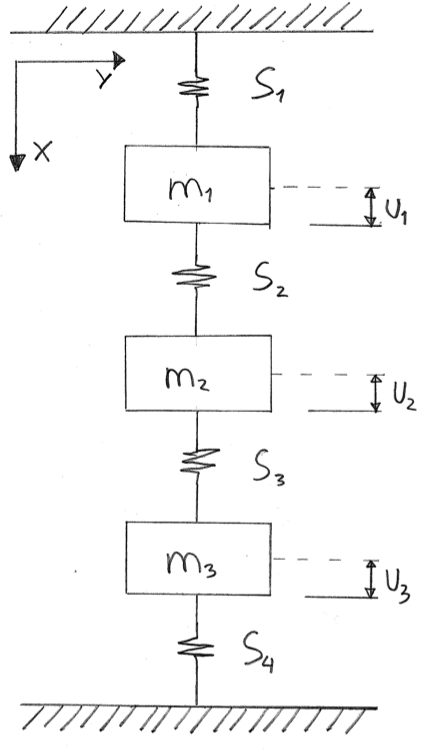
\includegraphics[width=6cm]{./images/equilibrium_framework_basic_spring_mass_problem.png}
\caption{Basic spring mass problem.}
\label{fig:basic_spring_mass_problem}
\end{figure}

Let's start by labeling the various quantities acting in the
system. The three masses are represented by $m_1$, $m_2$, and $m_3$. 
The masses are connected by spring $s_1$, $s_2$, $s_3$, and $s_4$.
Gravity $g$ acts on each mass hereby defining the external
forces $f_1$, $f_2$, and $f_3$, defined to be positive downwards. 
The displacement of the masses, due to the forces acting on them, is represented
by $u_1$, $u_2$, and $u_3$. \\ 

When the gravitational force acts on the masses it causes each separate spring to
react. The internal spring forces are represented by $w_1$, $w_2$,
$w_3$, and $w_4$. A positive $w_i$ value is defined to be stretch and
a negative value is compression. For each spring we define a connecting quantity
$e_1$, $e_2$, $e_3$ and $e_4$ one for each elongation of the spring. \\


% The mass displacements $u_i$ and the internal spring forces $w_i$ are the primary
% unknowns we want to determine. There is some constitutive 
% law that connects the mass displacement $u_i$ to the internal
% spring force $w_i$. 

By using vectors to represent each of the quantities $u$, $e$, $w$ and
$f$ we can describe the problem by relating these as follows:

\begin{itemize}
\item There will be a matrix $A$ relating the displacement vector
$u$ to a elongation vector $e$.
\item There will be a matrix $C$ relating the elongation vector $e$
  to a spring force vector $w$.
\item There will be a matrix relating the spring force vector $w$ to the
  external force vector $f$. %, it happens that this final matrix is $A^T$.
\end{itemize}

\begin{figure}
  \centering
  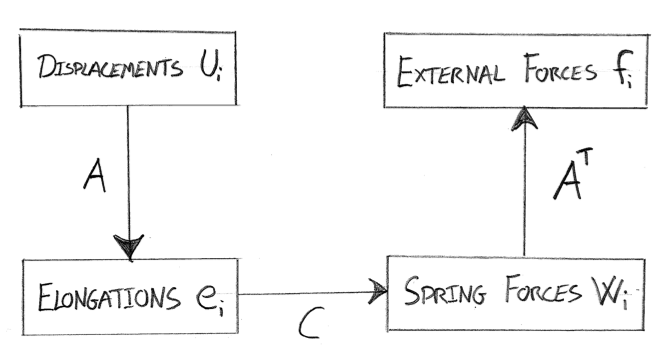
\includegraphics[width=10cm]{./images/equilibrium_framework_basic_ep_framework.png}
\caption{The structure of the framework.}
\label{fig:basic_ep_framework}
\end{figure}

% figure showing the main framework with 4 components
Figure \vref{fig:basic_ep_framework} illustrates how the different
quantities can be related by matrices. This is what forms the significant structure
of the framework used all over the field of applied mathematics. We
are about to describe the fundamental framework for
equilibrium steady state problems. \\

\subsection{Relating Displacements to Elongations}
We will begin by constructing matrix $A$. This is the question of
how much the springs stretch due to the displacement $u$. As seen
on figure \vref{fig:basic_spring_mass_problem} there are four springs
and three mass displacements. The relation between the two quantities
written on matrix form is:

\begin{equation}
\label{eq:e_related_to_u}
e = A \ u  
\end{equation}

where vector $e$ equals $[e_1, e_2, e_3, e_4]^T$, vector $u$ equals
$[u_1, u_2, u_3]^T$ and $A$ is the matrix relating the two quantities. 
The first spring $s_1$ stretches by the amount equal to the displacement of
the first mass. So $e_1 = u_1$ because the spring is fixed at
the top. The spring being fixed at one end introduces the first
boundary condition. Later it will become clear why 
boundary conditions, limiting the solution space, are an important
part of the framework. The elongation of the second spring
equals the displacement $u_2$ subtracted by $u_1$ because we are only interested in the stretching
of $s_2$. Looking at the third spring we isolate it by
subtracting the springs already stretched above therefore $e_3 = u_3 -
u_2$. The last spring $s_4$ is fixed at its end point causing it to
compress since it can not move further downwards. The amount it is
being compressed must be equal to the displacement of the last mass,
note the negative sign due to compression, therefore $e_4 = -u_3$. \\

The equations are:
\begin{align*}
e_1 &= u_1 \\
e_2 &= u_2 - u_1 \\
e_3 &= u_3 - u_2 \\
e_4 &= -u_3
\end{align*}

% Creating a $4 \times 1$ matrix for vector $e$ and a $3 \times 1$ matrix for
% vector $u$ we can create a $4 \times 3$ matrix and obtain the four $e$
% equations by matrix multiplication as stated by equation
% \vref{eq:e_related_to_u}. $e_1$ equals $u_1$ so the first row of matrix
% $A$ must be $[1, 0, 0]$ picking out the first element in $u$. Next we have
% $e_2 = u_2 - u_1$ equal to $-1$ times $u_1$ and $1$ times $u_2$,
% row 2 in matrix $A$ is therefore $[-1, 1, 0]$. In the third row we need
% $-1$ times $u_2$ and $1$ times $u_3$, this can be expressed as $[0,
% -1, 1]$. The last row in matrix $A$ is $[0, 0, -1]$ because $e_4 = -u_3$. \\

Written out in matrix form a certain pattern emerges

\begin{align}
\begin{bmatrix}
e_1 \\ e_2\\ e_3 \\ e_4
\end{bmatrix}
=
\begin{bmatrix}
 \phantom{-}1 & \phantom{-}0 & \phantom{-}0 \\
           -1 & \phantom{-}1 & \phantom{-}0 \\
 \phantom{-}0 &           -1 & \phantom{-}1 \\
 \phantom{-}0 & \phantom{-}0 &           -1
\end{bmatrix}
\begin{bmatrix}
u_1 \\ u_2 \\ u_3 \\
\end{bmatrix}
\end{align}

As we shall see later, matrix $A$ contains information about the
boundary conditions. In this example the boundary conditions are the
two fixed springs, the one at the top and the one at the bottom. \\


%\textbf{Step two}\\
\subsection{Relating Elongations to Spring Forces}
We will now determine matrix $C$. 
Matrix $C$ is the one that relates the distances the springs have
stretched to the internal spring forces $w$. Relating spring
extension to a force is exactly what Hooke's law does. Hooke's law as
defined in equation \eqref{eq:hooks_law} on page \pageref{eq:hooks_law}:

\begin{equation*}
f = -k \ \Delta x 
\end{equation*}

where $\Delta x$ is the distance the spring has been stretched or
compressed. $f$ is the restoring force and $k$ is the spring
constant defining units of force it takes to stretch or compress the
spring one unit length. The relation between the internal spring
forces $w$ and the spring elongation $e$ is written as:

\begin{equation}
\label{eq:w_related_to_e}
w = C \ e  
\end{equation}

where vector $w$ equals $[w_1, w_2, w_3, w_4]^T$, vector $e$ equals
$[e_1, e_2, e_3, e_4]^T$ and $C$ is the $4 \times 4$ matrix relating the two
quantities. Using Hooke's law we need to define a spring constant. When
the spring constant is multiplied with the stretch $e$ the internal
force $w$ are obtained. For each spring we define
a spring constants $c_1$, $c_2$, $c_3$ and $c_4$. The internal
spring forces is then obtained by:

\begin{align*}
w_1 &= c_1 e_1 \\
w_2 &= c_2 e_2 \\
w_3 &= c_3 e_3 \\
w_4 &= c_4 e_4
\end{align*}

Equation \eqref{eq:w_related_to_e} written on matrix form:

\begin{align}
\begin{bmatrix}
w_1 \\ w_2\\ w_3 \\ w_4
\end{bmatrix}
=
\begin{bmatrix}
c_1 &  &  &  \\
 & c_2 &  &  \\
 &  & c_3 &  \\
 &  &  & c_4 \\
\end{bmatrix}
\begin{bmatrix}
e_1 \\ e_2 \\ e_3 \\ e_4
\end{bmatrix}
\end{align}

where $0$ is implied in all the blank entries of the $4 \times 4$
matrix $C$. Note how we
just introduced an external law from the world of physics into the
framework. The physical law was here introduced as a relation between
two quantities in the framework. \\

%\textbf{Step three} \\
\subsection{Relating Spring Forces to External Forces}
The last relation that will take us all the way around the framework
is the one between the internal 
forces $w$ and the external forces $f$. This is where the state of
equilibrium is represented by a key equation, in this case the equation
describes the conservation of forces as described by definition
\vref{static-equilibrium}.\\

We need to find the relation between the internal and external
forces. When the system has reached its state of equilibrium all
springs and masses have stopped moving, therefore the internal and external
forces must cancel out. The only external force in this
system is the gravity acting on each of the three masses, obtained by:

\begin{equation}
\label{eq:force_eq_mass_times_gravity}
f_i = m_i \ g
\end{equation}

where $g$ is the gravity and $i \ \epsilon \ \lbrace 1,2,3
\rbrace$.\\

Consider figure \vref{fig:basic_spring_mass_problem} and look at the
first internal force $w_1$ defined at spring $s_1$. When the system is
in a state of equilibrium $w_1$ must cancel out the forces pulling
down mass $m_1$. There are two forces pulling down mass $m_1$, the first
one is $f_1$ as defined in equation
\eqref{eq:force_eq_mass_times_gravity}. The second one is all the 
other masses below which equals whatever spring $s_2$ is
holding defined by $w_2$. The first internal force $w_1$ is obtained by:

\begin{equation}  
\label{eq:w1_equal_e2_times_f1}
w_1 = f_1 + w_2
\end{equation}

which can be written as $w_1 - w_2 = f_1$. Now consider the internal
force $w_2$, both $f_2$ and $w_3$ act downwards, therefore $w2$ must
equal the sum of the contributions: $w_2 = f_2 +w_3$. The three relations
between the internal forces and the external forces is obtained by: 

\begin{align*}
w_1 - w_2 &= f_1 \\
w_2 - w_3 &= f_2 \\
w_3 - w_4 &= f_3
\end{align*}

On matrix form these relations can be expressed as:

\begin{align}
\begin{bmatrix}
f_1 \\ f_2\\ f_3
\end{bmatrix}
=
\begin{bmatrix}
  \phantom{-}1 &           -1 & \phantom{-}0 & \phantom{-}0 \\
  \phantom{-}0 & \phantom{-}1 &           -1 & \phantom{-}0 \\
  \phantom{-}0 & \phantom{-}0 & \phantom{-}1 &           -1 
\end{bmatrix}
\begin{bmatrix}
w_1 \\ w_2 \\ w_3 \\ w_4
\end{bmatrix}
\end{align}

This is the crucial moment where we realize that the matrix relating
the internal forces $w$ to the external forces $f$ is exactly
$A^T$ - and it always is. No matter what kind of equilibrium problem we
are trying to solve the structure as illustrated in figure
\vref{fig:basic_ep_framework} always appears. 

\begin{quote}
\defit{"Nature produced $A^T$ there - we just sort of watched it happen."}
(Gilbert Strang)
\end{quote}

The fact that the
relation between internal forces $w$ and external forces $f$ is the
transpose of the relation between the displacements $u$ and the
elongation $e$ is not by accident. What it means is: the change in
internal stored energy when stretching the springs equals the amount
of external work done at the masses (equation
\eqref{eq:external_work_equals_internal_energy} on page
\pageref{eq:external_work_equals_internal_energy}). \\  

%\textbf{Assembling the equations}\\
\section{Assembling the Equations}
The equation $e = A \ u$ formed matrix $A$ and the equation $f = A^T w$ formed $A^T$.
These two matrices appears from the geometry expressing how things are
connected, how mass $m_1$ is connected to mass $m_2$ and so forth.
There is always a matrix $C$ in the middle that represents the laws of
physics or engineering, statistics or some other external law
depending on the problem domain. \\

In this case the three equations that
took us around the framework were:

\begin{equation}
\label{eq:e_a_u}
e = A \ u 
\end{equation}

\begin{equation}
\label{eq:w_c_e}
w = C \ e 
\end{equation}

\begin{equation}
\label{eq:f_at_w}
f = A^T  w
\end{equation}

% By elimination of $w$ in equation \vref{eq:f_at_w} and elimination of
% $e$ in equation \vref{eq:w_c_e} 

By substitution we can assemble the three equations and
hereby obtain a single expression that connects forces $f$ and
displacements $u$:

\begin{equation}
\label{eq:f_eq_at_c_a_u}
f = A^T C A \ u
\end{equation}

The product of $A^T C A$ is what relates the input forces to the
resulting displacements. Figure \vref{fig:final_ep_framework}
illustrates the framework with the relations we have obtained.

% insert figure here
\begin{figure}
  \centering
  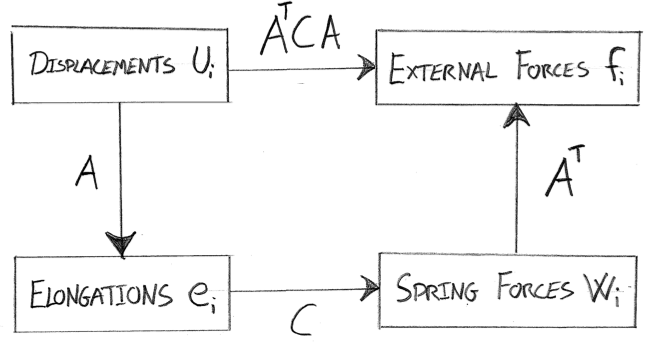
\includegraphics[width=10cm]{./images/equilibrium_framework_final_ep_framework.png}
\caption{The framework with relations connecting each quantity.}
\label{fig:final_ep_framework}
\end{figure}


Calculating the product of $A^T C A$ will
lead to a special matrix. From the spring and mass example the
following matrices were obtained:

\begin{equation*}
A^T = 
\begin{bmatrix}
  \phantom{-}1 &           -1 & \phantom{-}0 & \phantom{-}0 \\
  \phantom{-}0 & \phantom{-}1 &           -1 & \phantom{-}0 \\
  \phantom{-}0 & \phantom{-}0 & \phantom{-}1 &           -1 
\end{bmatrix}
\ \ \ \ \ \
A = 
\begin{bmatrix}
 \phantom{-}1 & \phantom{-}0 & \phantom{-}0 \\
           -1 & \phantom{-}1 & \phantom{-}0 \\
 \phantom{-}0 &           -1 & \phantom{-}1 \\
 \phantom{-}0 & \phantom{-}0 &           -1
\end{bmatrix}
\ \ \ \ \ \
C =
\begin{bmatrix}
c_1 &  &  &  \\
 & c_2 &  &  \\
 &  & c_3 &  \\
 &  &  & c_4 \\
\end{bmatrix}
\end{equation*}

Multiplying the $3 \times 4$ matrix $A^T$ by the $4 \times 4$ matrix
$C$ and then multiplying the result by the $4 \times 3$ matrix $A$ equals
a $3 \times 3$ matrix:

\begin{equation*}
\begin{bmatrix}
  \phantom{-}1 &           -1 & \phantom{-}0 & \phantom{-}0 \\
  \phantom{-}0 & \phantom{-}1 &           -1 & \phantom{-}0 \\
  \phantom{-}0 & \phantom{-}0 & \phantom{-}1 &           -1 
\end{bmatrix}
\begin{bmatrix}
c_1 &  &  &  \\
 & c_2 &  &  \\
 &  & c_3 &  \\
 &  &  & c_4 \\
\end{bmatrix}
\begin{bmatrix}
 \phantom{-}1 & \phantom{-}0 & \phantom{-}0 \\
           -1 & \phantom{-}1 & \phantom{-}0 \\
 \phantom{-}0 &           -1 & \phantom{-}1 \\
 \phantom{-}0 & \phantom{-}0 &           -1
\end{bmatrix}
=
\begin{bmatrix}
 c_1 + c_2 & -c_2       &            \\
      -c_2 &  c_2 + c_3 &       -c_3 \\
           &       -c_3 &  c_3 + c_4 \\
\end{bmatrix}
\end{equation*}

%\textbf{Stiffness matrix}\\
\section{The Stiffness Matrix}
\label{sec:the-stiffness-matrix}
The matrix $A^T C A$ represents the connections and their properties
in the system. In the domain of solid
mechanics matrix $A^T C A$ is also known as the 
\defit{stiffness} matrix. The stiffness matrix $K$ with spring constant
$c_i = 1$ corresponding to the
system as illustrated in
figure \vref{fig:basic_spring_mass_problem} is obtained by:

\begin{equation*}
K =
\begin{bmatrix}
 c_1 + c_2 & -c_2       &            \\
      -c_2 &  c_2 + c_3 &       -c_3 \\
           &       -c_3 &  c_3 + c_4 \\
\end{bmatrix}
= 
\begin{bmatrix}
 \phantom{-}2 &           -1 & \phantom{-}0 \\
           -1 & \phantom{-}2 &           -1 \\
 \phantom{-}0 &           -1 & \phantom{-}2 \\
\end{bmatrix}
\end{equation*}

%\textbf{Positive definite stiffness matrix}\\
\subsection{Positive Definite Stiffness Matrix}
The resulting matrix $K$ has some interesting properties. First of all it
is invertible. Remember it is the matrix that relates the displacement
to the forces so physically it should be invertible because the system is well
defined, so if the forces were known we could determine the
displacements and the other way around. Secondly it is \textit{positive
definite} defined by \citebook{page~18}{book:applied_math}:

\begin{definition}
A is positive definite if $f = x^T A x$ is always positive (for $x \neq 0$) 
\end{definition}

where $A$ is a matrix and $x$ is a vector. In our case we are interested in showing
that the stiffness matrix $K$, where $K = A^T C A$, is positive
definite, this can be expressed as: 

\begin{equation}
\label{eq:pos_definite}
x^T A^T C A \ x > 0 
\end{equation}

To prove that it is positive
definite consider equation \eqref{eq:pos_definite}. Vector $x$ can be
any vector so if it equals the displacement vector $u$ we obtain $A
\ u$ which equals $e$ as defined in equation \eqref{eq:e_a_u}.  
The transpose of $A \ x$ is $x^T A^T$ so equation
\eqref{eq:pos_definite} can also be written as:

\begin{equation}
\label{eq:et_c_e}
e^T C \ e > 0 
\end{equation}

By taking the product of $e^T C \ e$ we obtain:

\begin{equation*}
\begin{bmatrix}
e_1 & e_2 & e_3 & e_4
\end{bmatrix}
\begin{bmatrix}
c_1 &  &  &  \\
 & c_2 &  &  \\
 &  & c_3 &  \\
 &  &  & c_4 \\
\end{bmatrix}
\begin{bmatrix}
e_1 \\ e_2\\ e_3 \\ e_4
\end{bmatrix}
=
\begin{bmatrix}
c_1 e_1^2 + c_2 e_2^2 + c_3 e_3^2 + c_4 e_4^2
\end{bmatrix}
\end{equation*}

due to the square of $e$ the equation always comes out positive as long as the spring
constants are positive (which they are by definition). 
%By integrating
%over $e$ in Hooke's law defined in equation 
%\vref{eq:hooks_law}
The potential energy in a spring can be obtained by
\citebook{page~175}{book:uni-physics}:

\begin{equation}
\label{eq:hooks_potential_energy}
E_U = \frac{1}{2} k \Delta x^2
\end{equation}

where $k$ is the spring constant ($c_i$) and $\Delta x$ is the stretch ($e_i$),
multiplying equation \eqref{eq:et_c_e} by $\frac{1}{2}$ we realise that
the following is an expression of the potential energy in the springs

\begin{equation}
\frac{1}{2}c_1 e_1^2 + \frac{1}{2}c_2 e_2^2 + \frac{1}{2}c_3 e_3^2 +
\frac{1}{2}c_4 e_4^2 =
\frac{1}{2}e^TCe 
\end{equation}

Not only did we prove $A^T C A$ to be positive
definite, $A \ x = 0$ only in the case where $x=0$, we also
showed that this equation is the relation between forces $f$ and
displacements $u$, this leads to the important point that whenever
there is movement, the potential energy is positive. 
%
$A \ x = 0$ only in the case where $x=0$ so when there is no movement
($x=0$), which is the case in the initial configuration, the potential
energy equals $0$.\\ 


%\textbf{Positive semi-definite stiffness matrix}\\
\subsection{Positive Semi-definite Stiffness Matrix}
The expression $A^T C A$ took us around the framework, in this
case it represents an
energy and was proved positive definite. The matrix $A$ and its
transpose was constructed from the geometry of the problem. To see why
the stiffness matrix $K$ has to be positive 
definite consider the stiffness matrix of the system illustrated in 
figure \vref{fig:unbound_spring_mass_problem}. Here we have three masses
($n=3$) connected by two springs ($m=2$). None of the springs are
fixed so there are no boundary conditions. 

\begin{figure}
  \centering
  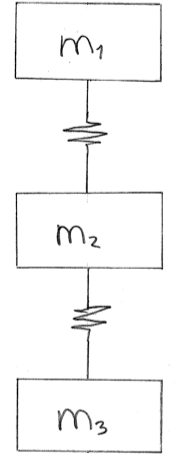
\includegraphics[width=2cm]{./images/equilibrium_framework_unbound_spring_mass_problem.png}
\caption{Spring mass problem without boundary conditions.}
\label{fig:unbound_spring_mass_problem}
\end{figure}
 
Recall how matrix $A$ was constructed, it is going to be a $n \times m$
matrix where the first
row represents the stretching in the first spring.
% Here being $-1$ of
% the top displacement in mass $m_1$, $1$ for the displacement of mass
% $m_2$ and $0$ for mass $m_3$ because this is not connected to
% $m_1$. The first row is
% therefore $[-1, 1, 0]^T$. 
Matrix $A$ for this problem becomes:

\begin{equation*}
A =
\begin{bmatrix}
           -1 & \phantom{-}1 & \phantom{-}0 \\
 \phantom{-}0 &           -1 & \phantom{-}1 
\end{bmatrix}
\end{equation*}

The stiffness matrix $K = A^T C A$ with each spring constant
equal to $1$ is obtained by

\begin{equation*}
K =
\begin{bmatrix}
            -1 & \phantom{-}0 \\
  \phantom{-}1 & -1 \\
  \phantom{-}0 & \phantom{-}1
\end{bmatrix}
\begin{bmatrix}
 1 &   &   &   \\
   & 1 &   &   \\
   &   & 1 &   \\
   &   &   & 1 \\
\end{bmatrix}
\begin{bmatrix}
           -1 & \phantom{-}1 & \phantom{-}0 \\
 \phantom{-}0 &           -1 & \phantom{-}1 
\end{bmatrix}
= 
\begin{bmatrix}
 \phantom{-}1 &           -1 & \phantom{-}0 \\
           -1 & \phantom{-}2 &           -1 \\
 \phantom{-}0 &           -1 & \phantom{-}1 \\
\end{bmatrix}
\end{equation*}

Here matrix $K$ is only semi-positive definite which means 

\begin{equation}
\label{eq:semi_pos_definite}
x^T A^T C A \ x \geq 0 
\end{equation}

where $x$ is any non-zero vector. So for instance

\begin{equation*}
\begin{bmatrix}
 \phantom{-}1 &           -1 & \phantom{-}0 \\
           -1 & \phantom{-}2 &           -1 \\
 \phantom{-}0 &           -1 & \phantom{-}1 \\
\end{bmatrix}
\begin{bmatrix}
 1 \\ 1 \\ 1 
\end{bmatrix}
= 
\begin{bmatrix}
 0 \\ 0 \\ 0 
\end{bmatrix}
\end{equation*}

so clearly matrix $K$ can take a non-zero vector to
the \defit{null space}. In this case it goes for all multiples of the vector
$[1,1,1]^T$. Assume that vector $x$ is equal the displacement vector $u$, we are free to
move all masses arbitrarily by the same amount, up or down, without causing any
change in the potential energy. This is an example of a system that is not well defined
due to the missing boundary conditions. \\

% As established in equation \vref{eq:f_eq_at_c_a_u} displacements $u$
% are related to forces through the stiffness matrix $K$, so
% equation \vref{eq:f_eq_at_c_a_u} can be written as

% \begin{equation}
% f = K u
% \end{equation}

% Recognised to be the most important equation in steady state
% problems. The most important equation in dynamic problems is based
% upon the static case but now there is motion. According to Newtons law
% mass times acceleration is introduces as motion. So by introducing this into the
% equation we obtain

% \begin{equation}
% f = K u + M \ddot{u}
% \end{equation}
  
% where $K$ is the stiffness matrix, $u$ is the displacement vector, $M$
% is the mass matrix and $\ddot{u}$ is the acceleration equal to the
% second derivatives of the displacement. Often a damping
% term is also added to the equation. Dynamic problems will be discussed in
% details in section \vref{some_section}. \\

%estimation of stresses, displacements and structural analysis. 

Describing the element connections, finding the equations
and setting up the structure of the framework as explained here, is
exactly what the \defit{finite element method} is all about. 
The finite element method is one of the most powerful methods for
conducting structural analysis. It is used not
just in mechanics but all over the field of applied
mathematics. \\




 

